\section{Results}

\subsection*{Correlations}

\begin{itemize}
	\item Only 8 out of 42 plots were monotonic and allowed the use of  ``Spearman's rank correlation coefficient"
	\item Low or negative correlations
\end{itemize}

\textbf{Conclusion:} \textcolor{red}{\textbf{Inability to establish convergent validity}}

\clearpage

\subsection*{Same questions} 

%\begin{table} [H]
%	\begin{tabular}{| p{1cm} | p{1.5cm} | p{1.5cm} | p{2cm} | p{1.5cm} | p{1.5cm} |} \hline
%		Group & Frequency & p-value & Group & Frequency & p-value \\ \hline
%		G1 & 12 & 0.5271 & G2 & 9 & 0.2404 \\ \hline
%		G3 & 7 & 0.3837 & G4 & 8 & 0.6715 \\ \hline
%		G5 & 12 & 0.503 & G6 & 16 & 0.01523 \\ \hline
%		G7 & 13 & 0.1654 & G8 & 12 & 0.2984 \\ \hline
%		G9 & 10 & 0.1865 & G10 & 13 & 0.6893 \\ \hline
%		G11 & 19 & 0.3246 & G12 & 16 & 0.2246 \\ \hline
%		G13 & 30 & NA & G14 & 18 & 1 \\ \hline
%		G15 & 13 & 0.4957 & G16 & 12 & 0.0007 \\ \hline
%		G17 & 6 & 0.0522 & & & \\ \hline
%	\end{tabular}
%	\caption{Frequency and p-value of Same Answers}
%	\label{table:answers_frequency}
%\end{table}

\begin{figure}[H]
\centering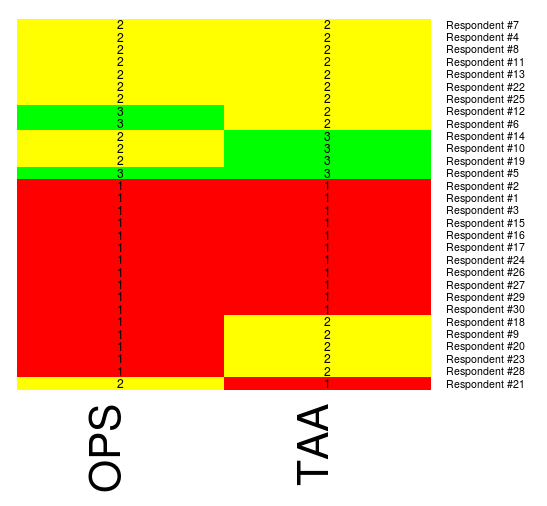
\includegraphics[width=0.5\linewidth]{../include/appendix/heatmaps/TestDrivenDevelopment}
\label{fig:tdd_heatmap}
\caption{Test Driven Development Heatmap}
\end{figure}

\clearpage

The p-values from the majority of the groups are more than the alpha level of 0.05. As a result, we cannot reject the $H_0$ hypothesis ({\scriptsize \textit{There is no difference between the groups of the same questions}}).

Nevertheless, as we see in Figure \ref{fig:tdd_heatmap} 1, the frequency of questions which are the same is low, thus, we consider the results as non-significant.

\textbf{Conclusion:} \textcolor{red}{\textbf{Questions which are the same among the tools don't yield the same results}}

\clearpage

\subsection*{Tools' Agile Practices Coverage}

\begin{table} [H]
\centering
	\scriptsize
	\begin{tabular}{| c | c | c | c |} \hline
		\textbf{Practice} & \textbf{TAA} & \textbf{PAM} & \textbf{OPS} \\ \hline
		Product Backlog & 2 & & 3 \\ \hline
		Smaller and Frequent Product Releases & 1 & 1 & 4 \\ \hline
		Constant Velocity & 1 & & \\ \hline
		Iteration Progress Tracking and Reporting & 17 & 5 & 5 \\ \hline
		Self-Organizing Teams & 11 & 1 & 7 \\ \hline
		Daily Progress Tracking Meetings & 1 & 5 & 1 \\ \hline
		Retrospective Meetings & 5 & 6 & 4 \\ \hline
		Test Driven Development & 3 & 3 & 4 \\ \hline
		Refactoring & 2 & 1 & 4 \\ \hline
		Software Configuration Management & 1 & & 1 \\ \hline
		Adherence to Standards & 3 & & 2 \\ \hline
		Continuous Integration & 5 & 5 & 10 \\ \hline	
		Evolutionary Requirements & & & 4 \\ \hline
		\textbf{Total} & 52 & 26 & 49 \\ \hline
	\end{tabular}
	\caption{{\footnotesize Agile Practices Coverage By Tools Based on Laurie Williams' Case Studies}}
\end{table}

\clearpage

\begin{table} [H]
\centering
	\footnotesize
	\begin{tabular}{| c | c | c | c |} \hline
		\textbf{Practice} & \textbf{TAA} & \textbf{PAM} & \textbf{OPS} \\ \hline
		Iterative and Incremental Development & 2 & 5 & 3 \\ \hline		
		Customer/User Acceptance Testing & & 5 & \\ \hline		
		Appropriate Distribution of Expertise & 2 & & 5 \\ \hline
		High-Bandwidth Communication & 4 & 8 & 13 \\ \hline					
		Client-Driven Iterations & & 2 & 3 \\ \hline
		Minimal or Just Enough Documentation & & & 4 \\ \hline
		Continuous Feedback & & 1 & 2 \\ \hline
		\textbf{Total} & 8 & 21 & 30 \\ \hline
	\end{tabular}
	\caption{{\footnotesize Agile Practices Coverage By Tools Excluding The Ones from Laurie Williams' Case Studies}}
\end{table}

\clearpage

\begin{table}
\centering
	\begin{tabular}{| c | c |} \hline
		\textbf{Ordered by practices} & \textbf{Ordered by questions} \\ \hline
		OPS (18) & TAA (52) \\ \hline
		TAA (15) & OPS (49) \\ \hline
		PAM (13) & PAM (26) \\ \hline
	\end{tabular}
	\caption{Summary Of Agile Practice's Coverage}
	\label{table:agile_practices_coverage_summary}
\end{table}

\textbf{Conclusion:} \textcolor{red}{\textbf{The tools don't cover the same agile practices and to the same extent}} \\

\clearpage